\documentclass[letterpaper]{article}
\usepackage{underscore}
\usepackage[left=2.0cm, right=2.0cm, top=2.0cm]{geometry}
\usepackage[utf8]{inputenc}
\usepackage{graphicx}
\usepackage{graphics}
\usepackage[spanish]{babel}
\usepackage{lipsum}
\usepackage{float}
\usepackage{subfigure}

\title{EV\_2\_4\_giro\_de\_un\_motor\_de\_corriente\_directa.}
\author{Alcantar Diaz Joel Alejandro.}
\date{15/10/2019}

\begin{document}

\maketitle
\vspace{2cm}
\begin{center}
    
\includegraphics[scale=0.5]{IMG/UPZMG.png}\\
    \vspace{2cm}
    \begin{large}
        Universidad Politecnica de la Zona Metropolitana de Guadalajara. $\|$ $4^{to}$ A
    \end{large}
\end{center}
\vspace{2cm}\newpage
\section{Motor de corriente continua.}
Un motor de corriente continua funciona de tal forma en la que el rotor, que es un electro iman, se repele con los imanes permanentes del stator, esto genera una repulcion continua por las bobinas y causa el giro del rotor dependeindo del voltaje y la potencia del electro iman. Esto es gracias a que las escobillas tocan el colector, tambien llamado comutador, \\
En la figura 1 se puede ver de manera sencilla las partes internas del motor y su funcionamiento.\\
\begin{figure}[hpbt]
    \centering
    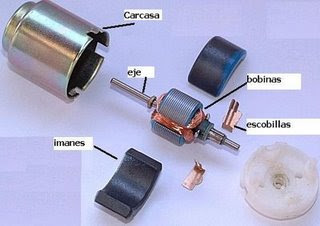
\includegraphics{IMG/mot.jpg}
    \caption{Partes de un motor con escobillas.}
    \label{fig:my_label}
\end{figure}
\section{Giro de un motor.}
Hay varias maneras de hacer girar un motor, aqui se enumeran las 2 principales.
\begin{enumerate}
    \item \textbf{Giro comun.}\\
    Consiste en simplemente conectar el motor de las dos maneras posibles.\\
    Es la manera mas simple pero al mismo tiempo la mas laboriosa ya que para invertir el giro se requiere de cambiar la instalación como se muestra en la figura 2.\\
    \begin{figure}[htbp]
        \centering
        \subfigure[Giro hacia la derecha]{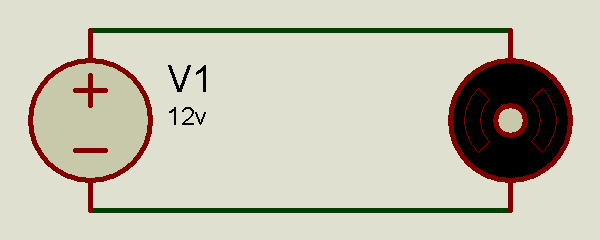
\includegraphics[scale=0.5]{IMG/motor.png}}
        \subfigure[Giro hacia la izquierda]{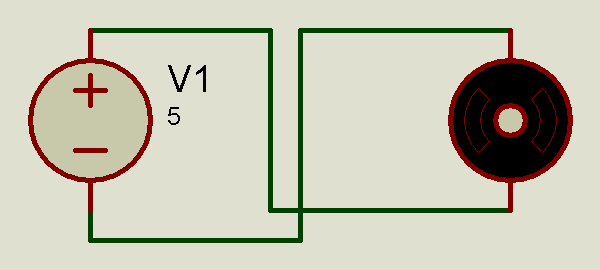
\includegraphics[scale=0.5]{IMG/motor2.png}}
        \caption{Cambio de giro simple.}
        \label{fig:motor_gir1}
    \end{figure}
    \item \textbf{Giro con puente H}\\
    El giro con un puente H consiste es 4 tranciatores, mosfet o 2 relevadores que al darle la señal invierten la corriente que se le suministra al motor, tambien es conocido como $"$Giro mediante interruptores$"$.
    \begin{figure}[htbp]
        \centering
        \subfigure[Puente H (aplica para mosfet y trancistores)]{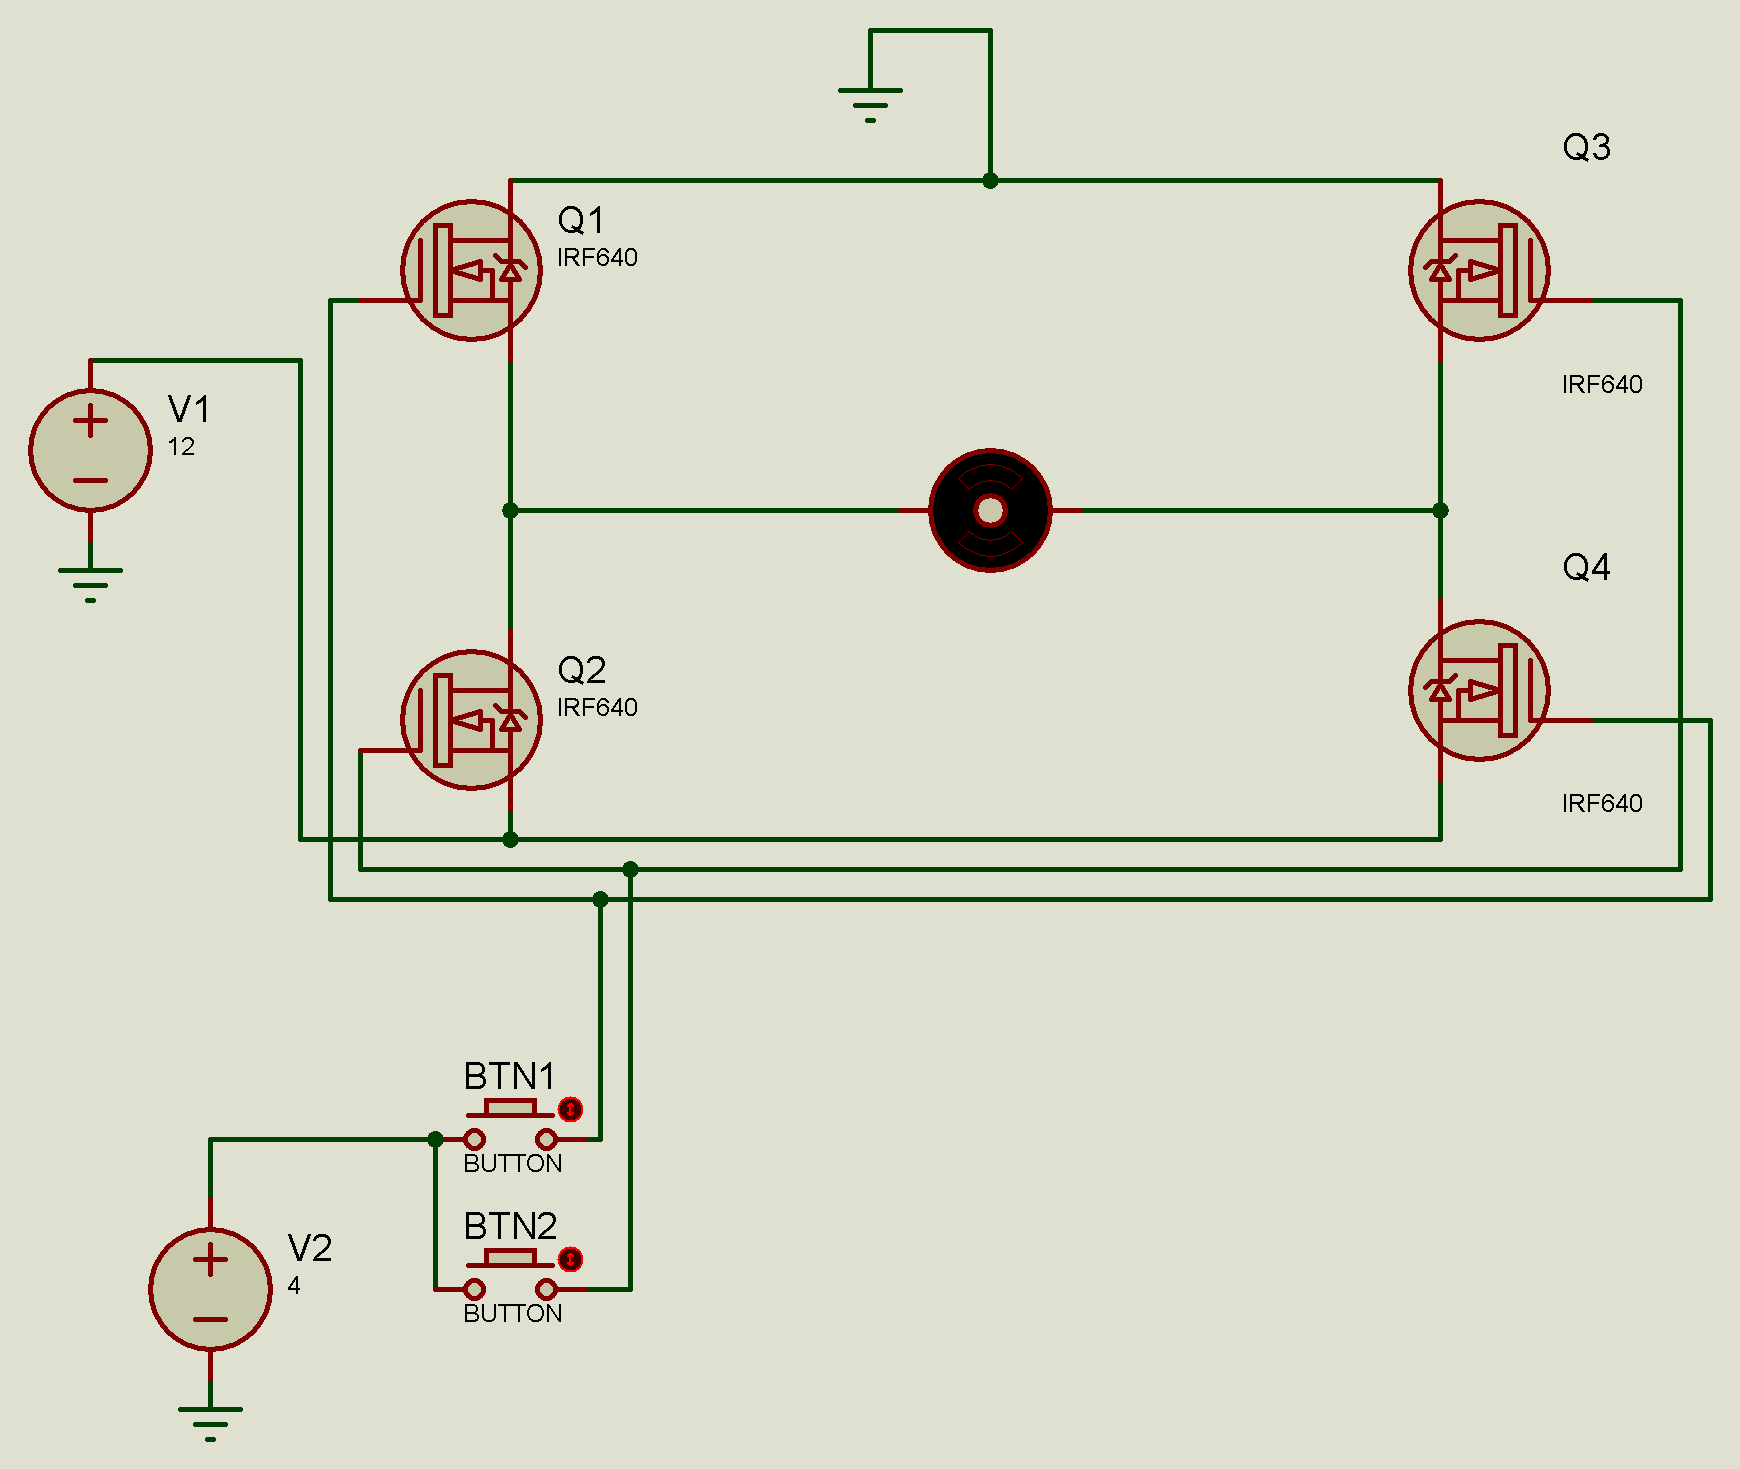
\includegraphics[scale=0.2]{IMG/puenteh.png}}
        \subfigure[Puente H con relay]{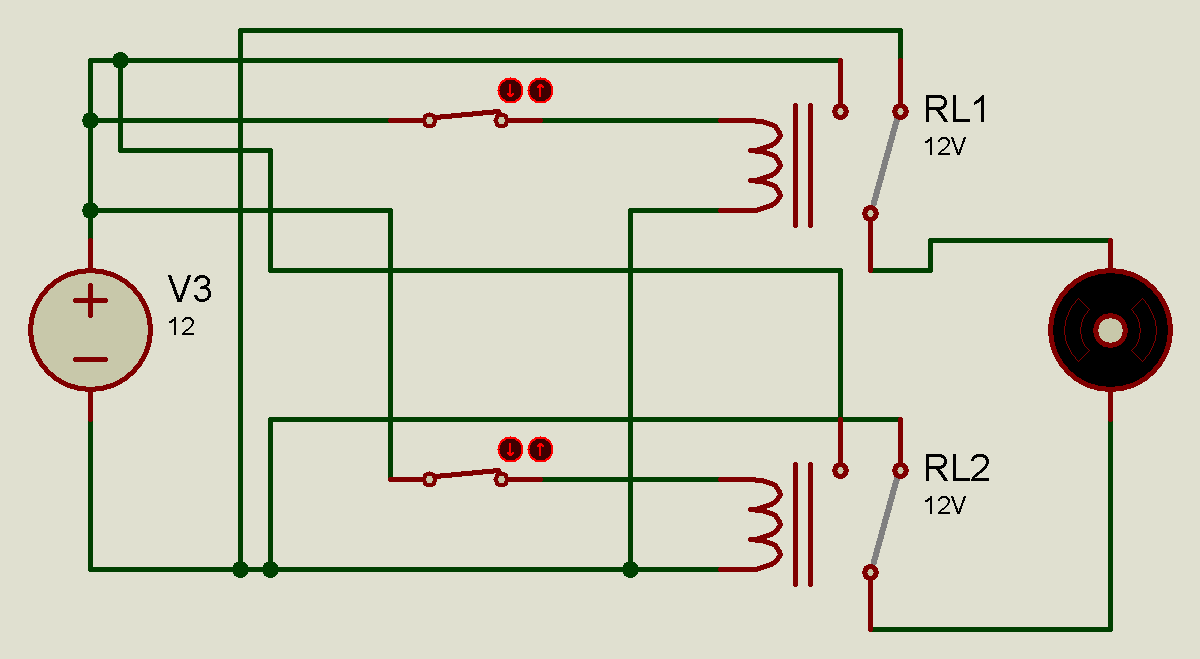
\includegraphics[scale=0.4]{IMG/puentehrel.png}}
        \caption{Caption}
        \label{fig:my_label}
    \end{figure}
\end{enumerate}
\end{document}
